\section{Post-weld Results}

\subsection{Magnetic results}

In order to investigate the effects that welding have on the magnetic performance of the material, samples at differing degrees of processing were taken and tested. An unaltered Vacoflux 17 wire was tested, as were a welded sample and two annealed ones.

The magnetic characterization of the samples consisted of a VSM test performed at the TU Delft 3ME laboratory, where the sample was subjected to magnetic field from 2.1T to -2.1T (\autoref{fig:hysteresis_loop}). From the successful ring printed as shown in \autoref{fig:ring_2}, a cross-sectional sample was taken. From the uppermost layer of this cross-section, a 2x2x2 mm sample was cut, since this was the maximum sample volume for the VSM. The rest of the cross-section was split and used for annealing.

\begin{minipage}{\linewidth}
    \centering
    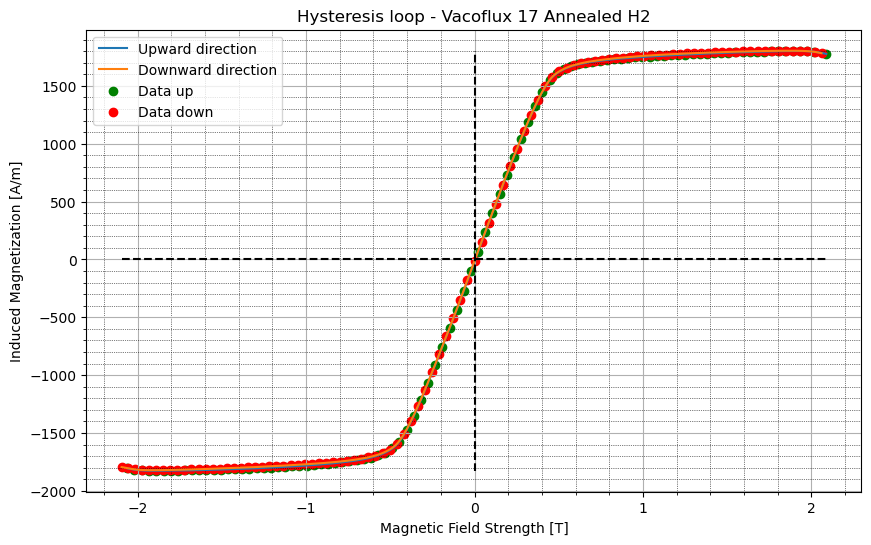
\includegraphics[width=\linewidth]{images/annealed_H2.png}
    \captionof{figure}{Hysteresis Loop of H$_2$ Annealed Sample }
    \label{fig:hysteresis_loop}
\end{minipage}

The recommended annealing is specified by the manufacturer in Vacoflux 17's data sheet as 850 C for 10 hours in a hydrogen atmosphere, followed by a cooling rate of 100-200 C/h. Hydrogen is relatively expensive and can cause leaks, so a first annealing with pure argon was attempted to verify whether the process could be performed by a cheaper and more stable gas. The second annealing was performed as intended by the manufacturer, using hydrogen.

Table 1 shows the relevant and testable parameters for the four conditions: as delivered by the manufacturer, and the three samples taken by the author. It is clear that the intended annealing provides significant improvement in the coercivity, remanence, and hysteresis loop area. For any kind of soft magnetic material, low coercivity, remanence, and iron losses (derived from the hysteresis loop area) are vital for performance as actuators or other components that need to be repeatedly magnetized and demagnetized. However, only a single slow hysteresis loop was evaluated, and tests at higher frequencies might be needed to gather the relevant data for the final application of the printed part.

The saturation magnetization suffers slightly, as does the maximum permeability (measured when no inducing field is applied). It must be said that the test conducted by the manufacturer measured the permeability for every level of induction, which was not the case here, and so the permeability results, which were calculated and not measured directly, should be interpreted with caution. The saturation magnetization is also not easy to compare with the manufacturer's claims, since one of the selling points of the material is a saturation induction of 2.2 T. Since the permeability at the saturation points in the VSM test are unknown, a direct comparison to the datasheet cannot be made, although welding and annealing showed to have little effect on the saturation magnetization of the sample. 

Broadly speaking, it can be said that the magnetic performance of Vacoflux 17 can be recovered and even improved upon through annealing after it has been welded using WAAM.

\subsection{Microscopy Results}

Still in progress.